\documentclass[a4paper]{book}
\usepackage[utf8]{inputenc}
\usepackage[english]{babel}
\usepackage{amsmath}
\usepackage{amsfonts}
\usepackage{amssymb}
\usepackage{color}
\usepackage{todonotes}
\usepackage{listings}
\usepackage{graphicx}
\usepackage{hyperref}
\definecolor{dkgreen}{rgb}{0,0.6,0}
\definecolor{gray}{rgb}{0.5,0.5,0.5}
\definecolor{mauve}{rgb}{0.58,0,0.82}

\newenvironment{mytheorem}[1]{\subsubsection*{Theorem #1}}{\begin{flushright}$\blacksquare$\end{flushright}}

\lstset{frame=tb,
  language=Java,
  aboveskip=3mm,
  belowskip=3mm,
  showstringspaces=false,
  columns=flexible,
  basicstyle={\small\ttfamily},
  numbers=none,
  numberstyle=\tiny\color{gray},
  keywordstyle=\color{blue},
  commentstyle=\color{dkgreen},
  stringstyle=\color{mauve},
  breaklines=true,
  breakatwhitespace=true
  tabsize=3
}
\author{Sandro Marcon}
\title{Riassunto DnA}
\begin{document}
\chapter{Introduzione}
\section{Notazione O-$\Omega$-$\Theta$ (pag 4)}
Per semplificare l'analisi asintotica degli algoritmi sono state introdotte le 
seguenti notazioni:

$$O(f)=\{ g|\exists a>0: \exists b>0: \forall N \in N : g(N)\leq af(N)+b \}$$
$$\Omega (f)=\{ g|\exists c>0: \exists \mbox{ infinite n } : g(n) \geq cf(n) \}$$
In entrambi i casi si tratta di classi di funzioni. Quando $f \in O(g)$ e $f \in \Omega (g)$ al contempo si dice che $f \in \Theta (g)$. Esistono ulteriori definizioni alternative, ad esempio quelle utilizzate nel Blatt 1. Il seguente teorema può essere utile (dimostrazione nel Blatt 1):
\newtheorem{theorem}{Theorem}
\begin{mytheorem}{1}
Date due funzioni $ f,g: N \rightarrow R^{+} $. Se $ \lim\limits_{x \rightarrow +\infty} \frac{f(n)}{g(n)} $ converge ad una costante $C\geq 0$ allora $f \in O(g)$.
\end{mytheorem}
\section{Algoritmo di Karatsuba (pag 12)}
Un esempio di algoritmo più efficiente per multiplicare due numeri è il seguente:
$$65 * 28 = (2 * 6) * 100 + (2 * 6) * 10 + (5 * 8) * 10 + 5 * 8 + (6-5)*(8-2) * 10 = 1820 $$
oppure, scritto in un altro modo:
\[ab*cd=100*a*c+10*a*c+10*b*d+b*d+10(a-b)(d-c)\]
In questo modo abbiamo solo 3 multiplicazioni elementari anziché 4. L'algoritmo può essere generalizzato grazie a divide and conquer dividendo ogni numero in due ed applicando l'algoritmo di base. Analizzando il tempo in base al numero delle multimplicazioni otteniamo che impieda circa $O(n^{1,58})$.
\section{Maximum subarray (pag 20)}
Dato un array di numeri il problema consiste nella ricerca del subarray con la somma degli elementi maggiore. Se essa è negativa il risultato è 0. Il metodo più efficiente per ricavare il risultato è il seguente:
\begin{lstlisting}
//A=array da 1, ... n	
max=0	
scan=0
for (i=1; i<=n; i++){	
	scan+=A[i]
	if scan < 0
		scan=0
	if scan > max 
		max=scan
}			
\end{lstlisting}
In questo modo il problema viene risolto in tempo lineare.	
\chapter{Sort}
Per semplicità ammettiamo che si debba sempre ordinare un array (chiamato $a$) contenente $n$ numeri (interi). In ogni caso con questi algoritmi è possibile ordinare qualsiasi oggetto appartenente ad un universo in cui vige un ordine totale.
\section{Sortieren durch Auswahl (pag 82)}
Selection sort consiste nel cercare ogni volta il minimo tra la posizione $i$ e $n$. Una volta trovato esso viene scambiato con l'$i-$tesimo numero. 
\subsubsection*{Esempio}
\[\begin{array}{*{20}{c}}
{}&{15}&2&{43}&{17}&4\\
{\Rightarrow}&2&{15}&{43}&{17}&4\\
{\Rightarrow}&2&4&{43}&{17}&{15}\\
{\Rightarrow}&2&4&{15}&{17}&{43}
\end{array}\]
\subsubsection*{Implementazione}
\begin{lstlisting}
int i,j, min, temp
for i=1:n-1
	min=i
	for j=(i+1):n
		if a[j]$<$ a[min]
			min=j
	temp=a[min]
	a[min]=a[i]
	a[i]=temp
\end{lstlisting}
\subsubsection*{Analisi}

Dal doppio loop si vede semplicemente che l'algoritmo impiega $\Theta (n^2)$ comparazioni e nel peggior caso (i numeri sono ordinati dal più grande al più piccolo) O(n) scambi. Da notare che per trovare il minimo sono necessari almeno $n-1$ confronti (Satz 2.1), quindi l'algoritmo non può andare più veloce di così. 
\section{Sortieren durch Einfügen (pag 85)}
In inglese si chiama insertion sort. Per induzione i numeri fino a $i-1$ sono già ordinati. Il principio consiste di piazzare l'$i-$tesimo elemento al giusto posto, se necessario scalando i restanti a destra di una posizione. Esempio:
\[\begin{array}{*{20}{c}}
{}&2&{15}&/&{43}&{17}&4\\
{\Rightarrow}&2&{15}&{43}&/&{17}&4\\
{\Rightarrow}&2&{15}&{17}&{43}&/&4\\
{\Rightarrow}&2&4&{15}&{17}&{43}&/
\end{array}\]
\subsubsection*{Implementazione}
\begin{lstlisting}
int i,j,t
for i=2:n
	j=i
	t=a[i]
	while a[j-1] > t
		//scala a destra di una posizione
		a[j]=a[j-1]
		j=j-1
	a[j]=t
\end{lstlisting}
Si nota subito che se implementato così l'algoritmo può non fermarsi se $t$ è il più piccolo numero. Serve quindi un elemento di stop, ad esempio inserendo $a[0]=t$ prima del while loop.

\subsubsection*{Analisi}

Nel peggior caso $\Theta (n^2)$ comparazioni ed altrettanti spostamenti. Nel miglior caso $O(n^2)$ comparazioni e spostamenti. Il caso medio rispecchia il peggiore.

\section{Bubblesort (pag 89)}
Il principio di questo algoritmo è semplicissimo: ad ogni iterazione viene scambiato l'elemento $a[i]$ con $a[i+1]$ (chiaramente solo se maggiore). In questo modo l'elemento più grande si sposta verso destra. Esempio:
\[\begin{array}{*{20}{c}}
{}&{15}&2&{43}&{17}&4\\
{\Rightarrow}&2&{15}&{43}&{17}&4\\
{\Rightarrow}&2&{15}&{17}&{43}&4\\
{\Rightarrow}&2&{15}&{17}&4&{43}\\
{\Rightarrow}&2&{15}&4&{17}&{43}\\
{\Rightarrow}&2&4&{15}&{17}&{43}
\end{array}\]
\subsubsection*{Implementazione}
\begin{lstlisting}
do
	flag=true
	for i=1:n-1
	if a[i] > a[i+1] 
		swap(a[i],a[i+1])
		flag=false
while (!flag)
\end{lstlisting}
\subsubsection*{Analisi}

Nel miglior caso, se l'array è già ordinato, abbiamo $n-1$ paragoni e nessuno scambio. Nel caso medio e peggiore l'algoritmo necessita di $\Theta (n^2)$ scambi e paragoni.

\section{Quicksort (pag 92)}
Il principio di quicksort è quello di scegliere un elemento come pivot (nel libro è sempre l'ultimo, ma ne basta uno casuale) e dividere l'array in due. A sinistra del pivot si trovano tutti gli elementi minori, mentre a destra quelli maggiori. Dopodiché viene richiamato l'algoritmo in modo ricorsivo sui due blocchi. L'algoritmo può essere eseguito ``in situ'', vale a dire che non serve spazio extra per salvare i dati (chiaramente un numero costante di variabili temporanee è permesso). Si usa quindi un solo array e si aggiungono due argomenti al metodo, ad esempio $l$ ed $r$, ad indicare l'intervallo in cui eseguire quicksort. Per dividere i numeri rispettivamente a destra ed a sinistra del pivot si può semplicemente far scorrere verso il centro due puntatori (chiamati $i$ e $j$) che partono rispettivamente alla posizione $l$ e $r$. Quando $a[i] \geq pivot$ e $a[j] \leq pivot$, $a[i]$ ed $a[j]$ vengono scambiati. Alla fine, quando $i=j$, l'elemento $a[i]$ viene scambiato col pivot e viene richiamato l'algoritmo da $l$ ad $i-1$ e da $i+1$ a $r$ (il pivot si trova già alla posizione giusta). Di seguito un esempio:
\subsubsection*{Esempio}
\begin{center}
array: 5 7 3 1 6 4\\
quicksort(array, 1, 6)
\end{center}
\[\begin{array}{*{20}{c}}
{}&{}&{}&5&7&3&1&6&{(4)}& \leftarrow &{{\text{pivot}}}\\
{}&{}&{}& \uparrow &{}&{}& \uparrow &{}&{}&{}&{}\\
{}&{}&{}&i&{}&{}&j&{}&{}&{}&{}\\
{}&{}& \Rightarrow &1&7&3&5&6&{(4)}&{}&{}\\
{}&{}&{}&{}& \uparrow & \uparrow &{}&{}&{}&{}&{}\\
{}&{}&{}&{}&i&j&{}&{}&{}&{}&{}\\
{}&{}& \Rightarrow &1&3&7&5&6&{(4)}&{}&{}\\
{}&{}&{}&{}&{}& \uparrow &{}&{}&{}&{}&{}\\
{}&{}&{}&{}&{}&{i,j}&{}&{}&{}&{}&{}\\
{}&{}& \Rightarrow &1&3&{(4)}&5&6&7&{}&{}
\end{array}\]
\begin{center}quicksort(array, 1, 2), quicksort(array, 3, 6)\end{center}
\subsection*{Implementazione}

\begin{lstlisting}
quicksort(int[ ] a, int l, int r)
	if r>l
		i=l-1
		j=r
		v=a[r] //pivot
		while (true)
			do
				i+=1
			until a[i]>=v
			do
				j-=1
			until  a[j]<=v
			if i>=j
				break
			swap(i, j) //scambia a[i] con a[j]
	 	swap(i,r)
		quicksort(a, l, i-1)
		quicksort(a, i+1, r)
\end{lstlisting}    
      
\subsection*{Analisi}
Nel peggior caso, ad esempio se la sequenza è già ordinata o più in generale se il pivot è sempre l'elemento maggiore o minore, quicksort impiega $O(n^2)$ comparazioni, poiché ad ogni ricorsione c'è un solo elemento in meno. In questo caso avverrebbero $O(n)$ spostamenti. Nel miglior caso l'algoritmo impiega un tempo di $\Theta (n\log (n))$, poiché l'albero delle ricorsioni ha un'altezza logaritmica. Lo stesso ragionamento vale per il numero di spostamenti. A pagina 99 c'è una lunga dimostrazione per induzione che mostra che anche il caso medio ha lo stesso tempo del miglior caso. Nonostante l'algoritmo sia in situ, anche le ricorsioni occupano un determinato spazio nella memoria, vale a dire $\Omega (n)$ chiamate. Rendendo l'algoritmo semi-iterativo si possono ottenere solo $O(\log (n))$ chiamate. Si deve semplicemente richiamare in modo ricorsivo quicksort sul più piccolo sub-array, mentre si completa l'altra parte in modo iterativo (algoritmo illustrato a pagina 100). Alla pagina successiva è invece mostrato come fare a rendere quicksort totalmente iterativo (personalmente non ho capito molto). 
            
\subsection*{Varianti di quicksort}
Per evitare un tempo di $O(n^2)$ nel caso di un array già ordinato sono state pensate alcune varianti dell'algoritmo, le quali concernono solamente la scelta del pivot. La prima è la cosiddetta 3-Median-Strategie (median of three values strategy), che consiste semplicemente nel prendere tre elementi campione, rispettivamente a destra, sinistra e nel mezzo, e scegliere come pivot il valore medio tra questi.
L'altra strategia si chiama Zufalls-Strategie (randomized quicksort) e consiste nel scegliere il pivot casualmente. Chiaramente può ancora avvenire un caso in cui necessita di un tempo quadratico, ma non esiste più una successione di numeri per cui questo accade. Una variante per rendere l'algoritmo glatt (smooth), cioè che impiega in media $O(n \log (n))$ comparazioni e  solo $O(n)$ quando l'input consiste in n elementi uguali, è la seguente. Praticamente gli elementi che sono uguali al pivot vengono spostati all'estrema destra o sinistra, dopodiché i due blocchi vengono riportati al centro e l'algoritmo prosegue come di consueto. L'implementazione ed una spiegazione più dettagliata possono essere trovate a pagina 104.

\section{Heapsort (pag 106)}
Heapsort si basa su insertion sort, ma invece di cercare il minimo/massimo ogni volta, che costa $O(n)$ paragoni, ci si affida ad un Heap (un tipo di albero binario). L'algoritmo è semplice ma efficace: finché l'albero non è vuoto si allontana la radice, nonché l'elemento massimo, e lo si scambia con l'ultimo elemento. Dopodiché tramite un indice si riduce l'albero di un elemento e si restaurano (tramite un metodo chiamato versickern) le sue proprietà (richiede un tempo di $O(\log (n))$). Rimane solo la parte iniziale, cioè la costruzione di un Heap a partire da un array qualsiaisi. Un metodo efficiente consiste nel eseguire il metodo ``versickern'' sulla sequenza delle chiavi $k_{\lfloor \frac{n}{2} \rfloor}, k_{\lfloor \frac{n}{2} \rfloor - 1}, ... , k_1$. Esempio:

\[\begin{array}{*{20}{c}}
{}&{2}&1&{5}&{3}&4&8&7&6\\
{\Rightarrow}&2&{1}&{5}&{6}&4&8&7&3\\
{\Rightarrow}&2&{1}&{8}&{6}&4&5&7&3\\
{\Rightarrow}&2&{6}&{8}&3&{4}&5&7&1\\
{\Rightarrow}&8&{6}&7&{3}&{4}&5&2&1\\
\end{array}\]

\subsection*{Implementazione}
\begin{lstlisting}
//costruiamo l'heap
for (i=n/2; i>=1; i--)
	versickere(a,i,n) //array a da i a N
//heapsort	
for (i=n	; i>=2; i--)
	swap(a[1],a[i])
	versickere(a,1,i-1)
\end{lstlisting}                                                                          
Dove versickere è:
\begin{lstlisting}
versickere(int[] a, int i, int m)
	int j
	while 2*i<=m //a[i] ha un figlio a sinistra
		j=2*i
		if j<m //a[i] ha anche un figlio a destra
			if a[j]<a[j+1]
				j=j+1
			//ora a[j] e' il figlio con un valore maggiore
			if a[i]<a[j]
				swap(a[i],a[j])
				i=j //va avanti a restaurare
			else
				i=m //fine		
\end{lstlisting}                                                                                                 
\subsection*{Analisi}
La costruzione dell'heap avviene in tempo lineare. Il resto dell'algoritmo prevede $n$ volte il metodo versickere, quindi in complesso l'algoritmo richiede $O(n \log (n))$ comparazioni e spostamenti nel peggior caso. Da notare che non occupa spazio extra, quindi è completamente ``in situ''. L'unico problema è che non è stabile, vale a dire che la posizione relativa di chiavi con lo stesso valore inizialmente adiacenti può cambiare. 

\section{Mergesort (pag 112)}
Anche mergesort si basa su divide and conquer. Si basa sul fatto che due blocchi dell'array sono già ordinati, quindi possono semplicemente essere uniti in tempo lineare, lasciando scorrere due indici nelle rispettive parti e salvando i valori in ordine crescente in un array temporaneo.

\subsection*{Esempio}
$A=\{2, 1, 3, 9, 5, 4\}$. Esso viene dunque diviso in due, vale a dire in $A_1 =\{2,1,3\}$ e $A_2 =\{9,5,4\}$. Per ricorsione essi vengono ordinati, quindi rimane da unire $A_1 =\{1,2,3\}$ e $A_2 =\{4,5,9\}$. Il passo merge prevede l'unione dei due insiemi, quindi si ottiene il risultato finale.

\subsection*{Implementazione}
\begin{lstlisting}
mergesort (int[] a, int l, int r)
	if l<r //altrimenti caso base: array rimane invariato
		m=(l+r)/2 //posizione media
		mergesort (a, l, m)
		mergesort (a, m+1, r)
		merge (a, l, m, r)
		
merge (int[] a, int l,m,r)
	i=l
	j=m+1
	k=l
	while (i<=m && j<=r)
		if a[i]<a[j]
			b[k]=a[i]
			i++
		else
			b[k]=a[j]
			j++
		k++
	if i>m //prima successione esautita
		for h=j:r
			b[k+h-j]=a[h]
	else
		for h=i:m
			b[k+h-i]=a[h]
	for h=l:r
		a[h]=b[h] //salva nuovamente nell'array originale									
\end{lstlisting}
\subsection*{Analisi}
Merge impiega sempre $O(n)$ spostamenti e comparazioni. Dato che l'array viene sempre diviso in due, il metodo merge viene chiamato $\log(n)$ volte. In totale l'algoritmo impiega sempre $\Theta (n \log(n))$. L'unico problema è che serve sempre $O(n)$ spazio extra per salvare l'array di supporto.
\subsection*{Mergesort iterativo}
L'algoritmo può anche essere reso totalmente iterativo. Esso si chiama ``reines 2-Wege-Mergesort'' (straight 2-way merge sort). L'idea è quella di unire tramite il metodo merge intervalli sempre più grandi (esattamente il doppio) fino ad avere l'intero array completamente ordinato. Esempio:
\[\begin{array}{*{20}{c}}
{}&{2}&1&{3}&{9}&6&5\\
{\Rightarrow}&1&{2|}&{3}&{9|}&5&{6|}\\
{\Rightarrow}&1&{2}&{3}&{9|}&5&6\\
{\Rightarrow}&1&{2}&{3}&5&{6}&{9|}\\
\end{array}\]
\begin{lstlisting}
straightmergesort(int[] a, int l,r)
	int size, ll, mm, rr
	size=1
	while size<r-l+1
		rr=l-1 //gli elementi fino ad a[rr] incluso sono a posto
		while rr+size<r //fino che tutti non sono elaborati
			ll=rr+1 //bordo sinistro successione 1
			mm=ll+size-1 //bordo desto successione 1
			if mm+size<=r
				rr=mm+size
			else
				rr=r
			merge (a, ll, mm, rr)
		size=2*size				
\end{lstlisting}
Le performance sono identiche a prima, ma il metodo è completamente iterativo.
\subsection*{Mergesort naturale}
L'unica differenza da straight 2-way merge sort è che al posto di unire successioni di lunghezza arbitraria sfruttiamo successioni già ordinate alla partenza. Ad esempio:
\[\begin{array}{*{20}{c}}
{}&{2}&1&{3}&{6}&9&5\\
{\Rightarrow}&{2|}&{1}&{3}&{6}&{9|}&{5}\\
{\Rightarrow}&1&{2}&{3}&{6}&{9|}&{6|}\\
{\Rightarrow}&1&{2}&{3}&5&{6}&{9|}\\
\end{array}\]
A livello di implementazione dobbiamo soltanto aggiungere la ricerca delle successioni già ordinate.
\begin{lstlisting}
straightmergesort(int[] a, int l,r)
	int ll, mm, rr
	do
		rr=l-1
		while rr<r
			ll=rr+1
			mm=ll	
			while (mm<r && a[mm+1]>=a[mm])
				mm++
			if mm<r
				while (rr<r && a[rr+1]>=a[rr])
					rr++
				merge (a, ll, mm, rr)
			else
				rr=mm
	until ll=l								
\end{lstlisting}
In questo modo cambiano anche le performance dell'algoritmo. Compare difatti un best case, ad esempio quando l'input è già ordinato. In questo caso avremmo $\Theta (n)$ comparazioni e 0 spostamenti. Il caso medio ed il peggior caso rispecchiano invece straight merge sort, nonché le tempistiche della prima analisi.
\section{Radixsort (pag 121)}
Radixsort si basa sulla comparazione delle cifre dei rispettivi numeri. Noi tratteremo solo la forma duale, ma il tutto funziona con qualsiasi forma, compresa quella decimale. Ammettiamo sempre che esista una funzione $z(i,k)$ che ritorna l'$i-$tesima cifra a partire dalla meno significativa del numero $k$. Ad esempio $z(0,517)=7$ e $z(2, 517)=5$.
\subsection{Radix-exchange sort}
L'algoritmo segue un principio abbastanza simile a quicksort: tutti gli elementi il cui $i-$tesimo bit è 0 vanno a sinistra, mentre se è uno vanno a destra. Il modo più semplice è quello, come in quicksort, di far scorrere due puntatori verso il centro e scambiare i numeri che si trovano al posto sbagliato. Dopodiché si richiama l'algoritmo sull' $(i-1)-$tesimo bit e sulle due parti dell'array.
\subsubsection*{Esempio}
\[\begin{array}{*{20}{c}}
{}&{1011}&{0010}&{1101}&{0011}&{|3}\\
{\Rightarrow}&{0011}&{0010;}&{1101}&{1011;}&{|2}\\
{\Rightarrow}&{0011}&{0010;}&{1011;}&{1101;}&{|1}\\
{\Rightarrow}&{0011}&{0010;}&{1011;}&{1101;}&{|0}\\
{\Rightarrow}&{0010}&{0011}&{1011}&{1101}
\end{array}\]
\subsubsection*{Implementazione}
\begin{lstlisting}
radixexchangesort(int[] a, int l,r,b)
	int i,j
	if r>l
		i=l-1
		j=r+1
		while (true)
			do
				i++
			until
				z(b, a[i])=1 || i>=j
			do
				j--
			until
				z(b, a[j])=0 || i>=j
			if i>=j
				break
			swap (a[i], a[j])
		if b>0
			radixexchangesort(a, l, i-1, b-1)
			radixexchangesort(a, i, r, b-1)						
\end{lstlisting}
\subsection*{Analisi}
L'algoritmo viene richiamato al massimo $b$ volte ed ogni volta impiega $O(n)$ paragoni e movimenti. In totale impiega dunque $O(bn)$ (tempo pseudo polinomiale). Se $b> \log (n)$ radixsort non è l'algoritmo adeguato al problema.
\subsection{Fachverteilung}
Questo algoritmo viene spesso anche chiamato bucket sort, poiché vengono utilizzati dei bucket per ordinare i numeri. L'idea di base è semplice: per ordinare una serie di numeri con $m$ cifre si inizia ad ordinarli dividendoli in bucket rappresentanti la cifra, sempre da destra a sinistra, dal basso all'alto. Dopo uno step bisogna ``raccogliere'' nuovamente la sequenza dai bucket e rieseguire il procedimento con la cifra successiva. Dopo $m$ step la sequenza è ordinata. L'algoritmo può praticamente essere diviso in due parti, dividere e raccogliere.
\subsubsection*{Esempio}
Sequenza originale: 40, 13, 22, 54, 15, 28. Primo step:    
\[\begin{array}{*{20}{c}}
{40}&{ }&{22}&{13}&{54}&{15}&{ }&{ }&{28}&{ }\\
{F0}&{F1}&{F2}&{F3}&{F4}&{F5}&{F6}&{F7}&{F8}&{F9}\\
\end{array}\]
La sequenza provvisoria diventa 40, 22, 13, 54, 15, 28. Secondo step:
\[\begin{array}{*{20}{c}}
{ }&{15}&{28}&{ }&{ }&{ }&{ }&{ }&{ }&{ }\\
{ }&{13}&{22}&{ }&{40}&{54}&{ }&{ }&{ }&{ }\\
{F0}&{F1}&{F2}&{F3}&{F4}&{F5}&{F6}&{F7}&{F8}&{F9}\\
\end{array}\]
Il risultato finale, letto da sinistra a destra e dal basso all'alto è quindi: 13, 15, 22, 28, 40, 54.
\subsubsection*{Implementazione}
Un approcio naiv sarebbe quello di creare $m$ bucket di dimensione $n$, in modo che nel peggior caso tutti i valori starebbero in un solo bucket. Questo però comporterebbe a $O(mn)$ spazio extra, quando realmente ne serve solo $\Theta (n)$ (ci sono sempre esattamente $n$ elementi). Ci sono due possibili soluzioni al problema. La prima è di usare liste lineari dalla dimensione non fissa, la seconda è quella di sondare quanti elementi andranno in ciascun bucket e dividere un array di dimensione fissa in $m$ scompartimenti tramite degli indici di divisione (Verteilungszahlen). Analizziamo dapprima la prima possibilità:
\begin{lstlisting}
radixsort_list(int[] a)
	List<Integer>[] l=new List<Integer>[m]
	int i,j,t
	for j=0:m-1
		l[j]=new List<Integer>() //inizializza la lista
	for t=1:l-1
		//fase di divisione
		for i=1:n
			j=z(t,a[i])
			l[j].pushtail(a[i]) //aggiunge all'ultima posizione
		//fase di raccolta
		i=0
		for j=0:m-1
			while (!l[j].isEmpty())
				a[i]=l[j].pophead()
				i++
				
\end{lstlisting}

Adesso la possibilità utilizzando un sondaggio prima della fase di divisione:
\begin{lstlisting}
radixsort_sond(int[] a)
	int[] b //array di dimensione n, numerato da 1 a n
	int[] c //array di dimensione m, Verteilungszahlen, da 0 a m-1
	int i,j,t
	for t=0:l-1
		//sondaggio
		for i=0:m-1
			c[i]=0 //inizializzazione
		for i=1:n
			j=z(t,a[i])
			c[j]++ 
		//futuri indici dell'array b
		c[m-1]=n+1-c[m-1]
		for i=2:m
			c[m-i]=c[m-i+1]-c[m-i]
		//fase di divisione
		for i=1:n
			j=z(t,a[i])
			b[c[j]]=a[i]
			c[j]++
		//fase di raccolta
		for i=1:n
			a[i]=b[i]				
\end{lstlisting}
\subsection*{Analisi}
Entrambe le implementazioni richiedono $O(l(m+n))$ passaggi e memoria di $O(n+m)$.
\section{Untere Schranke (pag 153)}
Per ora tutti gli algoritmi che usano comparazioni (praticamente tutti tranne radix sort) impiegano almeno $\Omega (n \log (n))$. 
\begin{mytheorem}{2.4}
Ogni algoritmo di ordinamento impiega nel caso medio e nel caso peggiore almeno $\Omega (n \log (n))$ paragoni per ordinare $n$ chiavi.
\paragraph*{Dimostrazione}
Per dimostrare questo teorema valutiamo tutte le possibili $n!$ permutazioni di $n$ chiavi e le inseriamo in un albero binario. Inizialmente l'algoritmo generico non conosce nulla sulla permutazione corrente, ma man mano che compara le chiavi si sposta tra i rami fino a raggiungere la foglia contenente la giusta permutazione. Praticamente un nodo $i:j$ rappresenta una comparazione. Esso ha due figli: a sinistra se $a[i]<a[j]$ e a destra se $a[i] \geq a[j]$. Dato che ci sono $n!$ permutazioni possibili devono per forza esserci $n!$ foglie. Ora non ci rimane che dimostrare che l'altezza massima e media di un albero binario con $k$ foglie sia di almeno $log_2 (k)$. In questo caso avremmo:
$$ log (k!) \geq \log \left(\left(\frac{n}{2}\right)^{\frac{n}{2}}\right) = \frac{n}{2} \log \left(\frac{n}{2}\right) \in \Omega (n \log (n))$$
\end{mytheorem}
\begin{mytheorem}{2.4.1}
L'altezza massima e media di un albero binario con $k$ chiavi è di almeno $ log_2 (k)$.
\paragraph*{Dimostrazione}
La prima parte è triviale, in quanto un albero di altezza $t$ può avere al massimo $2^t$ foglie. La seconda parte viene dimostrata per assurdo. Sia $T$ il più piccolo albero per cui l'ipotesi non regge. $T$ ha $k$ foglie, dunque $k \geq 2$ e $T$ deve avere un Teilbaum $T_1$ con $k_1$ foglie a sinistra e $T_2$ con $k_2$ foglie a destra. Chiaramente $k_1+k_2=k$. Dato che sia $T_1$ sia $T_2$ sono più piccoli di $T$, allora le loro altezze medie devono essere maggiori di $log_2(k_1)$ e rispettivamente $log_2 (k_2)$. Ovviamente l'altezza media di $T$ deve essere maggiore di uno rispetto ai due Teilbäume. Quindi:
\begin{eqnarray}
 altezza media(T) &=&  \frac{k_1}{k}(\mbox{altezza media}(T_1)+1)+\frac{k_2}{k}(altezza media(T_2)+1)      \nonumber \\
   &\geq & \frac{k_1}{k}(log_2(k_1)+1)+\frac{k_2}{k}(log_2(k_2)+1) \nonumber \\
   &=&\frac{1}{k}(log_2(2k_1)+log_2(2k_2)) = f(k_1,k_2)
\end{eqnarray}
Secondo la condizione che $k_1+k_2=k$, $f$ assume valore minimo quando $k_1=k_2=\frac{k}{2}$ quindi:
$$ \mbox{altezza media}(T) \geq \frac{1}{k}\left(\frac{k}{2} log_2(k)+\frac{k}{2} log_2(k)\right)=log_2 (k)$$
Si incappa dunque in una contraddizione.
\end{mytheorem}
\chapter{Search}
\section{Auswahlproblem (pag 168)}
Il primo approcio nel cercare di trovare l'$i-$tesimo elemento più piccolo è quello di ordinare dapprima la sequenza per poi eliminare i primi $i-1$ elementi. In questo caso si ottiene un tempo di $O(n \log (n))$. Seguendo lo stesso principio di quicksort è però possibile arrivare alla soluzione in tempo lineare. Per l'implementazione faremo uso del metodo, simile a quello usato in quicksort:
\begin{lstlisting}
int dividi(int l,r, pivot)
	/* divide a[l], ... , a[r] in due gruppi
	   a[l], ..., a[m-1] sono < pivot
	   a[m], ..., a[m] sono >= pivot
	   restituisce il valore di m */
\end{lstlisting}
Una volta trovato $m$ abbiamo tre possibilità: la chiave si trova nel primo gruppo o nel secondo o l'abbiamo trovata.
\begin{lstlisting}
trova (int l,r,i)
	int m,v
	if r>l
		scegliere pivot v
		m=teile(l,r,v)
		if i<=m-l
			trova (l, m-1, i)
		else
			trova (m,r,i-m+l
	else
		//r=l, qundi i=1
		//l'elemento si trova nella posizione a[l]	 			
\end{lstlisting}
Se scegliamo male il pivot l'algoritmo impiega $\Omega (n^2)$ passi. Se invece il pivot divide l'array in $qn$ e $(1-q)n$ elementi, con $0.5<q<1$ impiega:
\begin{eqnarray}
T(n) &=& T(qn)+cn \nonumber \\
& \leq & cn \sum_{i=0}^{+\infty} q^i = cn \cdot\frac{1}{1-q} \in O(n)
\end{eqnarray}
Per scegliere il pivot adeguato si può usare l'algoritmo proposto da Blum, chiamato ``median of median strategy''.
\begin{enumerate}
\item (caso base) se $n<$costante calcola l'$i-$tesimo più piccolo elemento direttamente.
\item dividi gli $n$ elementi in $\lfloor \frac{n}{5} \rfloor$ gruppi di cinque elementi e un gruppo con i restanti. 
\item ordina questi gruppi (in tempo costante) e per ogni gruppo trova la mediana. Se il gruppo ha un numero pari di elementi scegli il più grosso degli elementi medi. 
\item applica l'algoritmo ricorsivamente alle $\lceil \frac{n}{5} \rceil$ mediane per trovare la mediana delle mediane.
\item utilizza quest'elemento come pivot e procedi normalmente.
\end{enumerate}
Questa strategia assicura che ci sono almeno 
$$ 3\left(\lceil \frac{1}{2} \lceil \frac{n}{5} \rceil \rceil -2\right) \geq \frac{3n}{10} -6$$
elementi più piccoli di $v$. Segue quindi che l'algoritmo deve essere richiamato al massimo $ \lceil \frac{7n}{10} + 6 \rceil$ volte ricorsivamente. Il tempo impiegato è dunque:
$$ T(n) \leq T\lceil \frac{n}{5} \rceil +T \lceil \frac{7n}{10} +6 \rceil + an \leq ... \leq cn \in O(n) $$
\section{Sequenzielle Suche (pag 173)}
Ammettiamo che le $n$ chiavi siano salvate in un array o in una lista. Il modo più semplice per sondare la sequenza è quello di controllare le $n$ chiavi fino ad a trovare l'elemento desiderato. Per fare in modo che l'algoritmo si fermi iniziamo dal fondo e mettiamo uno stopper alla posizione 0.
\begin{lstlisting}
sequentialsearch (int k)
	int i
	a[0]=k //stopper
	i=n+1
	do
		i--
	while a[i] != k
	if i != 0
		//a[i] elemento ricercato
	else
		//non esiste nessun elemento k		
\end{lstlisting} 
Chiaramente l'algoritmo impiega 0 passaggi nel miglior caso e $n$ nel peggiore. Nel caso medio:
$$ \frac{1}{n} \sum_{i=1}^n i = \frac{n+1}{2} \in O(n) $$
\section{Binäre Suche (pag 174)}
La ricerca binaria si basa su divide and conquer. Ammettendo di avere un array ordinato si può descrivere l'algoritmo come segue:
\begin{enumerate}
\item se la sequenza è vuota la ricerca finisce senza successo, altrimenti guarda l'elemento $a[m]$ (posizione media).
\item se $k < a[m]$ applica sulla sequenza $a[1],\dots, a[m-1]$ lo stesso procedimento.
\item se $k \geq a[m]$ applica sulla sequenza $a[m],\dots, a[n]$ lo stesso procedimento.
\item se $k = a[m]$ l'elemento è stato trovato.
\end{enumerate}
\begin{lstlisting}
binsearch(int l,r,k)
	int m=(l+r)/2
	if l > r
		//ricerca conclusa senza successo
	else
		if k < a[m]
			binsearch(l, m-1, k)
		else if k > a[m]
			binsearch(m+1, r, k)	
		else
			//a[m]=k, elemento trovato				
\end{lstlisting}
Un'altra variante iterativa è la seguente:
\begin{lstlisting}
binsearch(k)
	int m,l,r
	l=1
	r=n
	do
		m=(l+r)/2
		if k < a[m]
			r=m-1
		else
			l=m+1
	until
		k=a[m] || l>r
	if k=a[m]
		binsearch=m
	else
		binsearch=0								
\end{lstlisting}
In questo modo una ricerca non impiega più che $\lceil log_2(n+1) \rceil \in O(n) $ passaggi.
\section{Interpolationsuche (pag 179)}
Nella ricerca binaria scegliamo ogni volta l'elemento a metà dell'array come pivot. Non sempre si tratta di una buona idea. Ad esempio se cerchiamo nell'elenco telefonico ``Bernasconi'' non lo apriamo al centro. L'unica differenza dalla ricerca binaria è dunque la scelta della $m$:
$$m= \lceil l+ \frac{k-a[l]}{a[r]-a[l]}(r-l) \rceil$$
Nel miglior caso impieghiamo un numero di paragoni costante, ma nel caso medio $O(log_2(log_2(n))$ comparazioni. Perdiamo però a causa della maggiore complessità delle operazioni aritmetiche e nel caso sfortunato, in cui impiega $O(n)$ paragoni.
\section{Selbstanordnende lineare Liste (pag 180)}
Ammettiamo di avere una lista contenente $n$ chiavi. Per cercare e dunque accedere all'$i-$tesimo elemento impieghiamo $i$ paragoni. Avrebbe senso spostare gli elementi più ricercati all'inizio della lista. Consideriamo pertanto alcune strategie: 
\begin{itemize}
\item Move to front: l'elemento ricercato viene spostato all'inizio della lista
\item Transpose: l'elemento ricercato viene spostato una posizione all'indietro (scambiato con il vicino a sinistra)
\item Frequency count: ad ogni elemento viene abbinato un contatore. Inizialmente esso è 0 ma ad ogni accesso aumenta di un'unità. La lista viene sempre ordinata in modo che ogni $i$ contatori di frequenza (Häufigkeitszähler) siano ordinati in ordine decrescente. 
\end{itemize}
Qual'è la migliore strategia? Si può notare che la transpose strategy presenta alcuni problemi se si accede ogni volta ad elementi adiacenti in modo alternato, ad esempio $n,n-1,n,\dots$ In generale move to front è la tecnica migliore, anche perché non necessita di spazio extra (per salvare gli indici).
\begin{mytheorem}{3.2}
Per qualsiasi algoritmo $A$ di auto ordinamento di liste e per qualsiasi successione $s$ di $m$ operazioni d'accesso vale:
$$ C_{MF}(s) \leq 2C_A(s)+X_A(s)-F_A(s)-m $$
Dove $C$ indica i costi delle operazioni, $F$ il numero delle operazioni gratuite e $X$ il numero delle operazioni a pagamento. In altre parole move to front non può essere più di due volte peggio di qualsiasi altro algoritmo. La dimostrazione per analisi ammortizzata si trova da pagina 183 a 186.
\end{mytheorem}
\chapter{Hashing}
Al posto di salvare gli elementi in una lista e cercarli tramite comparazioni si può salvare ogni elemento ad un determinato indice e calcolare dove si trova in modo matematico. Questo è il principio di una hash table. La funzione che collega le chiavi all'indirizzo di allocamento ($m$ posizioni possibili) è detta Hashfunktion (hash function):
$$h: K \rightarrow \{0,..., m-1\}$$
Questa funzione non deve essere forzatamente iniettiva, difatti due chiavi con $h(k)=h(k')$ sono dette sinonimi. Quando questo accade succede però anche una collisione, che vedremo come trattare. Per una tabella di grandezza $m$ contenente $n$ chiavi definiamo $\alpha = \frac{n}{m} $ come il fattore di utilizzazione (Belegungsfaktor, utilization factor). Una buona hash function deve essere facile da computare ed evitare il maggior numero possibile di collisioni.
Nel nostro caso utilizziamo il cossiddeto Division-Rest-Methode, ma esistono anche altri metodi, quale la multiplicazione della chiave con un numero irrazionale. Comunque
$$ h(k)=k \mbox{ mod }m$$
Una buona scelta per $m$ è che sia un numero primo.
\section{Hashing perfetto ed universale}
Se il numero di chiavi possibili è minore alla grandezza della tabella e già conosciuto in partenza possiamo costruire una funzione di hashing iniettiva che evita qualsiasi collisione. In questo caso si parla di hashing perfetto (perfektes Hashing).
Nella maggior parte dei casi non sappiamo però se è possibile evitare collisioni. Sia $H$ una collezione finita di hash functions. $H$ si chiama universale se per ogni diversa coppia di chiavi $x$ e $y$ vale:
$$ \frac{\left|\{h\in H: h(x)=h(y)\}\right|}{|H|} \leq \frac{1}{m}$$
In altre parole $H$ è universale se per ogni coppia di chiavi differenti al massimo la $m-$esima parte delle funzioni porta ad una collisione. La probabilità che due chiavi collidano con una funzione di $H$ è dunque al massimo $1\over m$. Per una funzione $h$ e due chiavi $x$ e $y$ definiamo:
$$
\delta (x,y,h) =
\left\{
\begin{array}{rl}
1 & \mbox{ se h(x)=h(y) e } x\neq y  \\
0 & \mbox{ altrimenti}
\end{array}
\right.
$$
Per un insieme di chiavi $Y$, rispettivamente di funzioni $H$:
$$\delta (x,Y,h)= \sum_{y \in Y} \delta (x,y,h)$$
$$\delta (x,y,H)= \sum_{h \in H} \delta (x,y,h)$$
$H$ è universale quando per due differenti chiavi $x$ e $y$: $\delta (x,y,H) \leq \frac{|H|}{m}$.
Ammettiamo che vogliamo aggiungere la chiave $x$ ad un'hash table universale in cui è già stata salvata una successione $S$ di elementi. Calcoliamo quindi l'Erwartungswert (penso sia il numero di elementi che andrà a collidere con $x$, pf verificare):\todo{Verificare!}
\begin{eqnarray}
E[\delta (x,S,h)] &=& \frac{1}{|H|} \sum_{h \in H} \delta (x,S,h) \nonumber \\
&=& \frac{1}{|H|} \sum_{y \in S} \delta (x,y,H) \nonumber \\
&\leq & \frac{1}{|H|} \sum_{y \in S} \frac{|H|}{m} \nonumber \\
&=& \frac{|S|}{m}
\end{eqnarray}
Adesso dimostriamo che esiste una classe di funzioni hashing universali (tramite esempio).
\begin{mytheorem}{4.2}
Sia $|K|=p$ un numero primo e $a \in \{1, ..., p-1\},b \in \{0, ..., p-1\}$. La funzione $h_{a,b}: K \rightarrow \{0, ..., m-1\}$ viene definita nel modo seguente:
$$ h_{a,b}(x)=((ax+b) \mbox{ mod } p) \mbox{ mod } m$$
La classe di funzioni $H=\{h_{a,b} : 1\leq a < p \mbox{ e } 0\leq b <p\}$ è una classe universale di hash functions. Dimostrazione a pagina 197.
\end{mytheorem}
\section{Hashverfahren mit Verkettung der Überläufer (pag 198)}
Penso sia anche chiamato separate chaining. In ogni caso si tratta di un metodo per gestire le collisioni. Quando due chiavi collidono esse vengono semplicemente salvate in una lista. Questo metodo può essere implementato in due modi differenti, rispettivamente separate Verkettung der Überläufer e direkte Verkettung der Überläufer. Nel primo caso gli elementi della Hashtabelle hanno due campi, uno per il valore e l'altro per il puntatore, mentre nel secondo caso c'è solo un puntatore e tutti gli elementi vengono salvati in una lista esterna. In questo caso la tabella presenta dimensioni più piccole, poiché in ogni voce è salvato solo un puntatore.
\subsection*{Analisi}
Poniamo che un indirizzo $j$ abbia la stessa probabilità di essere scelto indipendentemente dagli altri, quindi $p(j)=\frac{1}{m} \mbox{ , } \forall j$. Con $C_n$' verrà indicato il tempo (in numero di elementi valutati) di una ricerca infruttuosa, mentre $C_n$ indica una ricerca in cui viene trovato un risultato. Nel caso della direkte Verkettung abbiamo:
$$ C_n '=\frac{n}{m}=\alpha $$
$$ C_n = 1+\frac{\alpha}{2} $$
Nell'altro caso cambia solo il tempo della ricerca infruttuosa:
$$C_n '=\alpha + e^{-\alpha} $$
I principali vantaggi di ``appendere'' una lista alle voci dell'hash table sono quelli della facilità di eliminare una voce e che in questo modo è possibile avere un Belegungsfaktor maggiore delle dimensioni della tabella. Il più grande svantaggio è invece rappresentato dal fatto che serve spazio extra oltre alla tabella stessa.
\section{Offene Hashverfahren}
Attenzione: da non confondere con open hashing (in inglese si dice open addressing). Questo metodo consiste nel salvare le chiavi in voci libere presenti nella tabella. Si introduce pertanto una nuova funzione $s$ in modo da creare una Sondierungsfolge per la ricerca di altri spazi liberi. Definiamo quindi una funzione $s(j,k)$ in funzione del numero di collisioni e della chiave. $k$ verrà dunque salvato alla posizione:
$$(h(k)-s(j,k))\mbox{ mod }m$$
Già a partire da questa definizione si può notare che l'allontanamento di una chiave è problematica. Ad esempio se $k'$ collide con $k$ esso verrà salvato in una voce differente. Eliminando $k$ risulta dunque impossibile ritrovare $k'$. La soluzione a questo problema è quella di indicare $k$ come eliminato senza però cancellarlo definitivamente finché non viene inserita una nuova chiave al suo posto.
\subsection*{Vocabolario}
\begin{itemize}
\item Search(k): inizia dall'indirizzo $i=h(k)$. Finché $t[i]$ non è libero o l'elemento non è stato trovato vai avanti ed aumenta $j$. Se si giunge in una casella libera la ricerca è infruttuosa.
\item Add(k): prima cerca $k$. Se è già stata inserita non fare nulla, altrimenti inseriscila nella prima posizione libera.
\item Delete(k): cerca $k$ e marca l'indirizzo $i$ come eliminato. 
\end{itemize}  
\begin{lstlisting}
//Array t
//Array mark

search(Dato ds)
	int i,j
	j=0 //collisioni
	do
		i=(h(ds.key)-s(j,ds.key)) mod m
		j++
	until
		t[i].key==ds.key || mark[i]==free
	if mark[i]=occupied
		ds.item=t[i].item
	else
		print ("Ricerca infruttuosa")
		
add (Dato ds)
	int i,j
	j=0 //collisioni
	do
		i=(h(ds.key)-s(j,ds.key)) mod m
		j++
	until
		mark[i] != occupied 
		//ammettiamo che la chiave non sia stata inserita in precedenza
	t[i]=ds
	mark[i]=occupied
	
delete (int k)
	int i,j
	j=0 //collisioni
	do
		i=(h(ds.key)-s(j,ds.key)) mod m
		j++
	until
		t[i].key==k || mark[i]==free
	if mark[i]=occupied
		mark[i]=deleted
	else
		print ("Chiave non presente")						
\end{lstlisting}
\subsection{Lineares Sondieren}
$$ s(j,k)=j $$
Abbastanza inefficiente, poiché grossi pezzi occupati tendono a crescere ancora di più, aumentando così il numero di collisioni.
$$C_n '=\frac{1}{2} \left(1+\frac{1}{(1-\alpha)^2}\right) $$
$$C_n =\frac{1}{2} \left(1+\frac{1}{(1-\alpha)}\right) $$
\subsection{Quadratisches Sondieren}
$$s(j,k)=\lceil \frac{j}{2} \rceil ^2(-1)^j$$
In questo modo si riesce a sondare molto più velocemente, ma il fenomeno del sekundäre Häufung (secondary clustering) influenza l'efficienza. Due sinonimi hanno difatti la stessa sequenza dunrante la ricerca proprio come nel lineares Sondieren.
$$C_n = 1+\ln \left( \frac{1}{1-\alpha}\right)-\frac{\alpha}{2}$$
$$C_n '= \frac{1}{1-\alpha}-\alpha +\ln \left( \frac{1}{1-\alpha}\right)$$
\subsection{Double hashing}
$$s(j,k)=jh'(k) $$
In cui $h'$ è una seconda hash function. Per scegliere una buona funzione $h'$ bisogna essere sicuri che il risultato non sia influenzato dal risultato della prima, quindi che abbiano probabilità disgiunte. Da ricordarsi che $h'(k) \neq 0$ e che non sia divisore di $m$. Normalmente i tempi sono i seguenti:
$$ C_n '= \frac{1}{1-\alpha} $$
$$ C_n = \frac{1}{\alpha} \ln \left(\frac{1}{1-\alpha}\right)$$
Grazie all'algoritmo di Brent è però possibile migliorare il tempo della ricerca con successo:
\begin{lstlisting}
//hh = la seconda hash function

BrentEinfuegen (Datensatz ds)
	int i, b, bb
	i=h(ds.key)
	while mark[i]=occupied
		b=(i-hh(ds.key)) mod m
		bb=(i-hh(t[i].key)) mod m
		if mark[b]==free || mark[bb]=occupied
			i=b
		else
			swap (da, t[i])
			i=bb
	t[i]=ds
	mark[i]=occupied			
\end{lstlisting}
Grazie a questo algoritmo il tempo diventa il seguente:
$$C_n = 1+\frac{\alpha}{2}+\frac{\alpha ^3}{4}+... <2,5$$
\section{Dynamische Hashverfahren}
\todo[inline]{voi sapete cosa hanno fatto, perché mi sembra impossibile che in mezza mattina abbiano coperto l'intero capitolo!?}
\chapter{Bäume}
A volte può essere molto utile simulare le seguenti strutture dati. Questo può essere fatto semplicemente visitando il sito: \url{http://www.cs.usfca.edu/~galles/visualization/Algorithms.html}.
\section{AVL-Tree (pag. 284)}
Abbiamo visto che un albero binario naturale può degradare ad una lista. In tal caso la ricerca di un elemento richiede un tempo pari a $\Theta (n)$, poiché l'altezza dell'albero diventa n e non più log(n). Gli alberi AVL mantengono invece questa proprietà: essi sono difatti nominati balancierte Binärbäume (self-balancing binary trees). La condizione di base è difatti che per ogni nodo dell'albero l'altezza del figlio sinistro differisce da quello destro di al massimo 1. Può essere dimostrato che un albero AVL di altezza h contiene al minimo n elementi, dove:
$$ n\geq F_{h+2} = 1,7171*1,618^h$$
Quindi risolvendo secondo l'altezza:
$$ h\leq 1,44 log_2 (n)+1 \in O(log(n))$$
\subsection*{Suchen}
È dunque chiaro che applicando la ricerca come in normali alberi binari ordinati si impiega sempre O(log(n)).
\subsection*{Einfügen}
Non è sempre detto che aggiungendo un elemento all'albero esso mantenga le sue proprietà AVL. Definiamo dunque:
$$ bal(p)=\mbox{ Altezza del sottoalbero di destra - altezza sottoalbero di sinistra}$$
Chiaramente $bal(p) \in \{-1,0,1\}$. Per inserire una nuova chiave facciamo innanzitutto una ricerca per quel valore. Se la chiave viene trovata non dobbiamo far nulla poiché è già presente nell'albero, altrimenti la ricerca finisce in una foglia vuota, rappresentante l'ipotetica posizione della chiave. Noi inseriamo la nuova chiave in quella posizione, dopodiché aggiustiamo le condizioni AVL chiamando la procedura upin(p), dove p è il padre della nuova chiave. La condizione di uscita dal metodo upin è che bal(p) diventi 0. In tutti gli altri casi il metodo viene applicato ricorsivamente fino alla radice, qunidi non più di O(log(n)) volte. Definiamo con pp il padre della chiave p. Ci sono due casi: p è il figlio sinistro di pp o il destro. Entrambi i casi sono analoghi, analizzeremo però il primo caso. Se le condizioni AVL continuano ad essere mantenute durante gli ``aggiornamenti'' della variabile bal, il tutto prosegue normalmente. Può però accadere che $|bal(pp)|>1$, quindi bisogna intervenire con una rotazione o una doppia rotazione:
\begin{center}
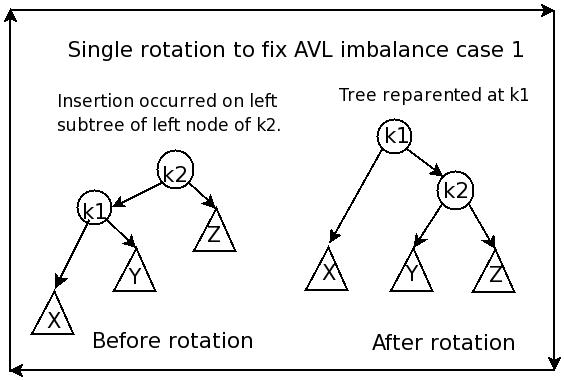
\includegraphics[scale=0.6]{Figures/singlerot.jpg}
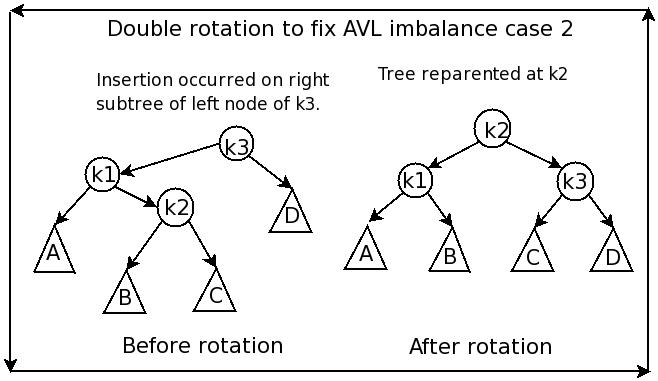
\includegraphics[scale=0.55]{Figures/doublerot.jpg}
\end{center}
\subsection*{Entfernen}
\begin{enumerate}
\item Se la chiave che si vuole allontanare non ha figli la si elimina direttamente e si chiama il metodo upout(p) al padre (analogo a upin)
\item Se la chiave p ha un solo figlio q per forza q non può avere figli. q prende quindi la posizione di p, dopodiché viene chiamato upout(pp).
\item Se p ha invece due figli si inverte la posizione di p con il suo successore/predecessore simmetrico finché la situazione non si riduce ad una precedente \todo{non ho capito bene, Fall 3 pag 293}. Anche in questo caso viene chiamato upout.
\end{enumerate}
Il metodo upout è analogo ad upin, cambia soltanto l'invariante (condizione d'uscita quando bal$(pp)=1$) e l'ordine delle rotazioni:
\begin{center}
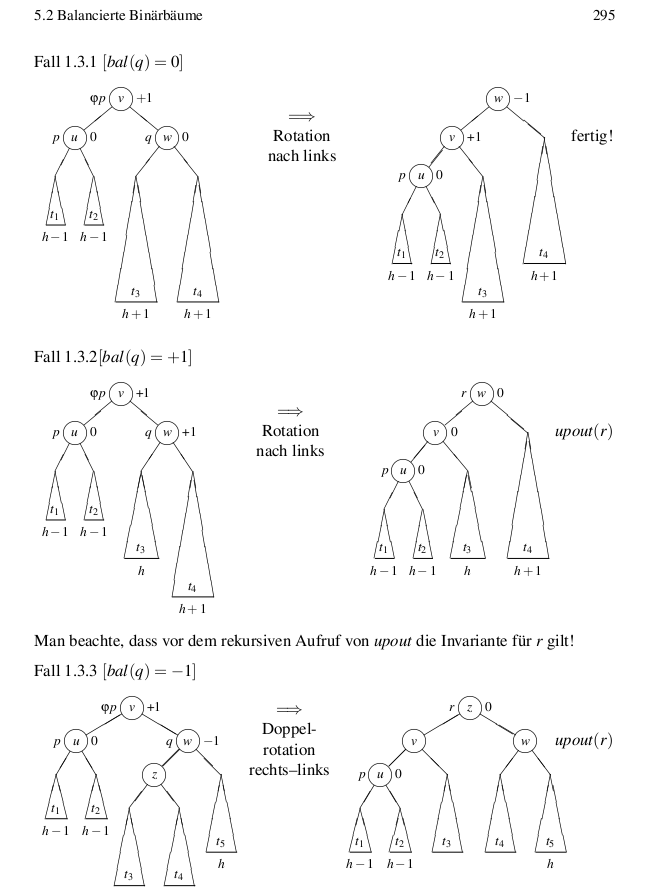
\includegraphics[scale=0.5]{Figures/avldeletion.png}
\end{center}
\section{Splay tree (pag. 328)}
Uno splay tree è un albero binario che può essere visto come una variante di move to front, poiché l'ultima chiave inserita, cercata o eliminata (se non c'è nell'albero viene sostituita dal padre) viene sempre resa radice (move to root strategy) grazie all'operazione splay(x). Quest'ultima è definita nella seguente maniera:
\begin{enumerate}
\item Cerca x nell'albero. Sia p il nodo in cui finisce la ricerca, altrimenti il padre della foglia nel caso di una ricerca infruttuosa.
\item Ripeti le seguenti operazioni di ordinamento (zig, zig-zig, zig-zag) finché p non diventa la radice.
\end{enumerate}
Non ci resta che elencare le operazioni:
\begin{center}
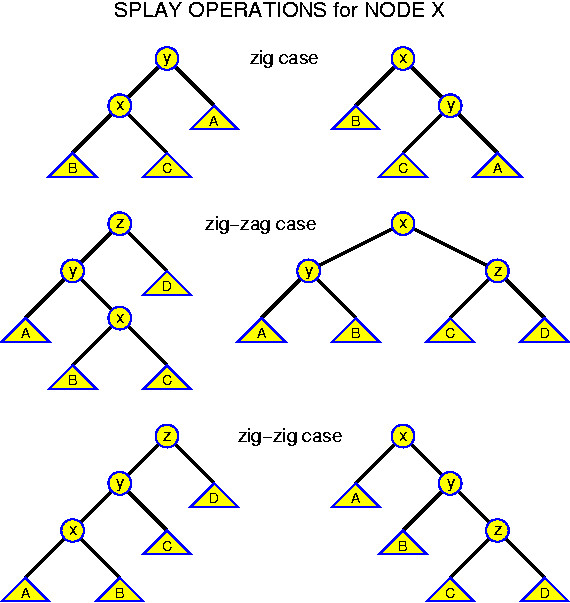
\includegraphics[scale=0.5]{Figures/splay.jpg}
\end{center}
\subsection*{Vocabolario}
\begin{itemize}
\item Inserisci(x): eseguire innanzitutto splay(x). Se la radice è x non fare niente, poiché la chiave è già presente nell'albero. Altrimenti nella radice si trova una chiave y che è il precedente/successivo simmetrico di x. Piazza dunque x come radice ed y come figlio sinistro rispettivamente destro.
\item Allontana(x): splay(x). Se la radice non è uguale ad x l'elemento non appartiene all'albero, altrimenti x si trova alla radice. Elimina dunque x e cerca la chiave più grande nel sottoalbero di sinistra (può essere fatto con splay($\infty$)). 
\item Cerca(x): splay(x). Se la radice è x l'elemento è stato trovato, altrimenti no.
\end{itemize}
Un'analisi ammortizzata, descritta completamente nel capitolo 5.4.2, porta al seguente teorema.
\begin{mytheorem}{5.1}
L'esecuzione di qualsiasi sequenza di m operazioni, in cui compare al massimo n volte inserisci, su uno splay tree inizialmente vuoto costa $O(m\log (n))$. 
\end{mytheorem}
\section{Optimal binary search tree (pag. 377)}
In questo caso abbiamo i seguenti valori (che non cambiano nel tempo) e vogliamo costruire un albero di ricerca ottimale:
\begin{itemize}
\item $S=\{k_1,k_2, ..., k_n \}$ insieme di n chiavi, dove $k_1<k_2<...<k_n$.
\item $a_i$ la probabilità assoluta che venga cercato $k_i$.
\item $I=(k_0,k_{n+1})$ intervallo in cui appartengono le chiavi.
\item $b_j$ probabilità assoluta che venga cercato un $x \in (k_j, k_{j+1})$, quindi che non venga trovato.
\end{itemize}
Definiamo dunque il peso dell'albero come:
$$W=\sum_i a_i + \sum_j b_j$$
La gewichtete Pfadlänge \todo{trovare traduzione decente} è invece:
$$ P= \sum_{i=1}^n (altezza(k_i)+1)a_i+\sum_{j=0}^n (altezza(foglia(k_i,k_{i+1}))b_j$$
Un albero di ricerca ottimale T è formato da sottoalberi anch'essi ottimali: 
$$ P(T)= P(T_l)+\mbox{peso della radice}+P(T_r)+W(T_l)+W(T_r)=P(T_l)+P(T_r)+W(T)$$
Se T è una foglia P(T)=0. Dividiamo dunque I in sempre più grossi intervalli fino ad ottenere l'albero ottimale secondo i principi della programmazione dinamica. Siano:
\begin{itemize}
\item T(i,j) l'albero ottimale per l'intervallo $(k_i,k_{j+1})$.
\item W(i,j) il peso di T(i,j), dunque $W(i,j)=b_i+a_{i+1}+...+a_j+b_j$.
\item P(i,j) la gewichtete Pfadlänge die T(i,j).
\end{itemize}
Grazie alla formula precedente si può calcolare P(i,j) utilizzando l'indice l della radice di T(i,j) e i due sottoalberi T(i,l-1) e T(l,j). Definendo:
$$W(i,i)=b_j$$
$$W(i,j)=W(i,j-1)+a_j+b_j$$
$$P(i,i)=0$$
$$P(i,j)=W(i,j)+\min_{i<l\leq j} \{P(i,l-1)+P(l,j)\}$$
e r(i,j) come gli indici delle radici di T(i,j) possiamo calcolare induttivamente su h=j-i (larghezza dell'albero) l'albero ottimale:
\begin{itemize}
\item h=j-i=0: T(i,i)=foglia ($k_i, k_{i+1}$). Poni W(i,i)=$b_i$, P(i,i)=0 e r(i,i) indefinito
\item h=j-i=1 $\rightarrow$ j=i+1. Dunque T(i,i+1) ha $k_{i+1}$ come radice. 

W(i,i+1)=W(i,i)+$a_{i+1}$+W(i+1,i+1)

P(i,i+1)=W(i,i+1)

r(i,i+1)=i+1
\item $h\geq 2$: $W(i,j)=W(i,l-1)+W(l,j)+a_l$

P(i,j)=P(i,l-1)+P(l,j)+W(i,j)

r(i,j)=l
\end{itemize}
Il procedimento elencato sopra necessita di $\Theta (n^2)$ di spazio. I casi con h=0 o h=1 possono essere completati in O(n), per il caso h>1:
\begin{lstlisting}
for h=2:n
	for i=0:(n-h)
		j=i+h
		/*trova la max l (i<l<=j) per cui
		P(i,l-1)+P(l,j) diventa minimo*/
		P(i,j)=P(i,l-1)+P(l,j)+W(i,j)
		r(i,j)=l		
\end{lstlisting}
Questo procedimento richiede un tempo di:
$$\sum_{h=2}^n \sum_{i=0}^{n-h} O(h+1)=\sum_{h=2}^n O((n-h+1)(h+1))= O(n^3)$$
Un possibile miglioramento deriva dal principio di monotonia, cioè:
$$r(i,j-1)\leq r(i,j) \leq r(i+1,j)$$
In questo modo la ricerca di l avviene semplicemente nell'intervallo $r(i,j-1)\leq l \leq r(i+1,j)$. In questo modo si può ridurre il tempo a $O(n^2)$. Per la dimostrazione e un esempio guardare a pagina 380-381.
In ogni caso non è sempre conveniente cercare un albero ottimale con questo algoritmo, a volte basta un albero quasi ottimale. Ad esempio nella serie 12 è stato calcolato un albero ottimale basandosi semplicemente sul fatto che la somma dei pesi di due sottoalberi sia minore della probabilità del nodo.
\begin{center}
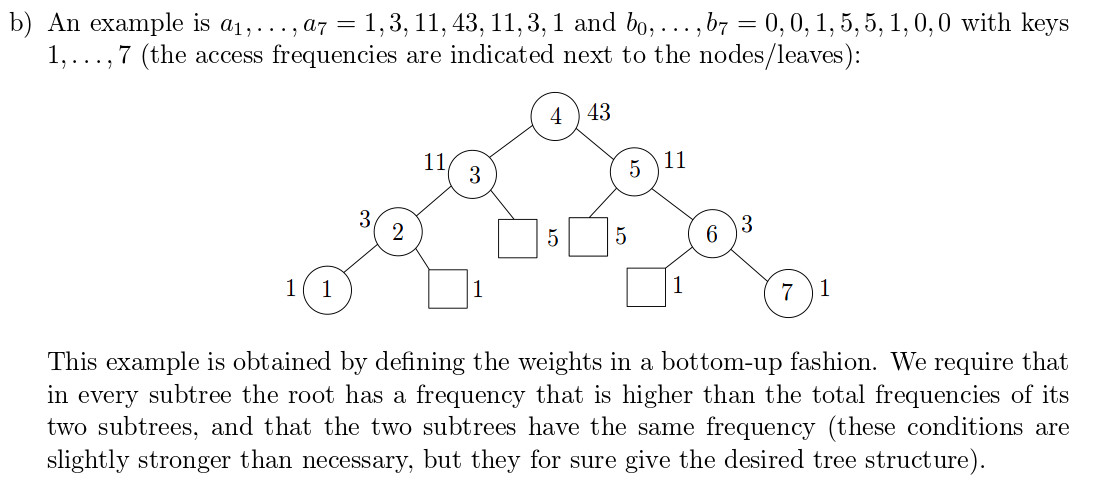
\includegraphics[scale=0.3]{Figures/optimaltree.jpg}
\end{center} 
\section{Binary Heap}
Abbiamo già in parte visto questa struttura per Heapsort. La sua principale caratteristica è che una chiave $k_i \leq k_{\lfloor\frac{1}{2} \rfloor}, 2\leq i\leq n$. In questo caso si tratta di un max Heap, se la relazione è al contrario si tratta di un min Heap. 
\paragraph*{Vocabolario}
A seguire l'implementazione di un min heap. Poniamo che le chiavi siano salvate in un array di dimensioni sufficienti. Salviamo inoltre la variabile n, che indica il numero di elementi presenti nell'array.
\begin{itemize}
\item Min: ritorna A[1]
\item Inserisci(x): incrementiamo n di uno e piazziamo x alla posizione A[n]. Per restaurare le proprietà dell'heap (x può essere minore del suo predecessore) chiamiamo bottom-up(i).
\item Delete(i): chiamiamo replace(i,A[n]). Dopodiché la chiave A[n] compare due volte, quindi riduciamo la dimensione dell'heap di uno. 
\item Replace(i,k): poniamo k'=A[i]. Innanzitutto A[i]=k, poi dobbiamo distinguere due casi: se k<k' chiamiamobottom-up(i), altrimenti shift-down(i). Da ricordarsi che shift-down(i) altro non è che versickere(i,n) trattato nel capitolo ``Sort''. In ogni caso è analogo a bottom-up(i).
\end{itemize}
\begin{lstlisting}
bottom-up(int i)
	while i>=2
		int j=i/2
		if A[j]<=A[i]
			break
		else
			swap(A[i],A[j])
			i=j	
\end{lstlisting}
\paragraph*{Analisi}
Ogni operazione del vocabolario può essere effettuata in tempo logaritmico.
\chapter{Manipolazioni di dati}
\section{Priority Queue (pag 404)}
Le priority queue (in tedesco dette Vorrangswarteschlangen) sono semplicemente delle code in cui ad ogni elemento è abbinata una priorità. Ad esempio chi ha il numero più basso passa prima di chi ha il numero più alto. Esse possono essere implementate in due differenti modi.
\paragraph*{Heap}
Il primo e più efficiente metodo è quello di usare un heap come una coda prioritaria. È possibile estrarre il minimo in tempo costante, inserire e rimuovere elementi in tempo logaritmico. L'unico problema è unire due heap. Questo può essere effettuato demolendo le strutture precedenti e creando un nuovo albero in O(n+k) passi.
\paragraph*{Lista}
Il metodo più intuitivo è forse quello di usare una semplice lista. Per unire due liste basta puntare il puntatore dell'ultimo elemento al primo della nuova lista. L'aggiunta di un nuovo elemento avviene in tempo costante, inserendolo o all'inizio o alla fine, mentre per rimuovere un elemento è necessario cercarlo in tutta la lista (quindi O(n)). La ricerca del minimo avviene anch'essa come nel caso della ricerca del massimo in un array, quindi in O(n). Una possibile variante è quella di ordinare gli elementi in ordine crescente. In questo caso il minimo può essere trovato in tempo costante, ma per inserire, rimuovere ed unire due liste si impiegherebbe O(n).
\section{Fibonacci heap (pag 420)}
I Fibonacci heap (anche chiamati F-Heap) sono collezioni di heap con insiemi di chiavi disgiunti. Le radici degli alberi sono collegate da una doppia lista lineare circolare. Ogni nodo ha un puntatore sul padre e su uno dei suoi figli. Inoltre i figli sono uniti da una doppia lista circolare. Il puntatore dell'heap indica direttamente l'elemento minimo, quindi la radice con il valore più piccolo.
\begin{lstlisting}
class HeapNode<Comparable>
	//parametri salvati
	HeapNode<E> destro, sinistro
	HeapNode<E> padre, figlio
	Comparable chiave
	int rango, marcato
\end{lstlisting}
\begin{center}
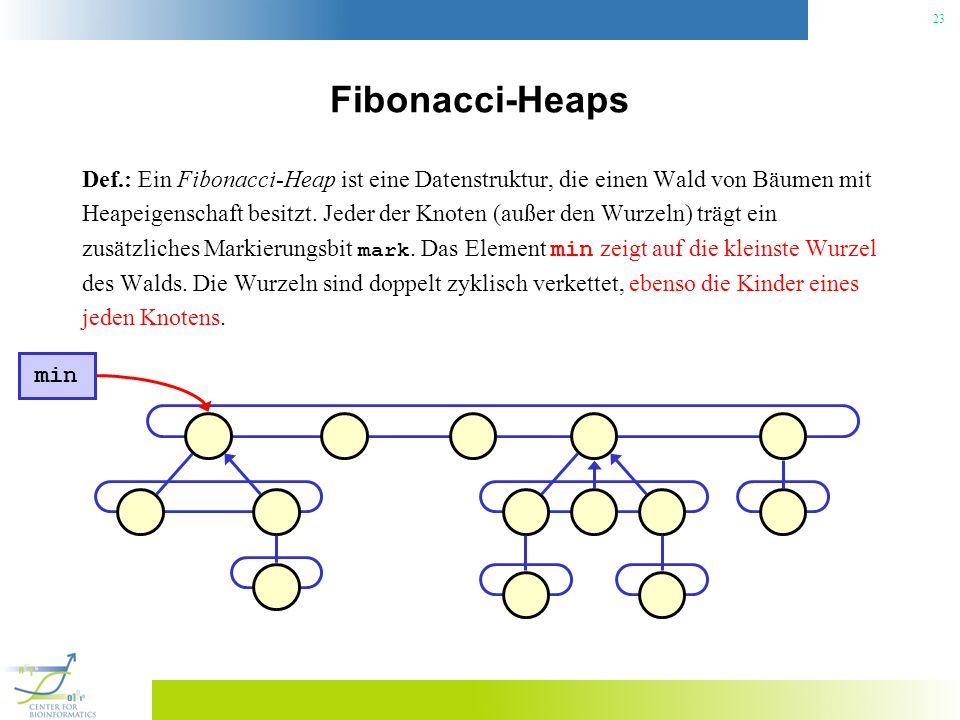
\includegraphics[scale=0.5]{Figures/fheap.jpg}
\end{center}
\subsection*{Vocabolario}
\paragraph*{Insert(x)} costruisci un F-Heap h' formato dalla sola chiave x ed uniscilo con h tramite meld(h').
\paragraph*{Min} il minimo è indicato dal puntatore dell'heap.
\paragraph*{Meld(h')} inserisci la radice di h' nella lista di radici di h. L'elemento più piccolo tra il minimo di h e quello di h' diventa l'elemento minimo del nuovo F-Heap.
Chiaramente le precedenti operazioni possono essere eseguite in tempo costante. 
\paragraph*{DeleteMin} I figli del minimo vengono inseriti nella lista delle radici, dopodiché il minimo viene rimosso. In seguito coppie di heap dallo stesso rango r vengono uniti in un heap dal rango r+1 (rendendo la radice più grande figlia di quella più piccola) finché nella Wurzelliste non rimangono più heap dallo stesso rango. Richiede O(log(n)).
\paragraph*{Decrease-key(x,k)} Diminuiamo il valore della chiave x con k.
\begin{lstlisting}
FIB-HEAP-DECREASE-KEY(H,x,k) 
	if k > key[x]
		//error "new key is greater than current key"
	key[x]=k
	y=p[x] //padre di x
	if y!=null && key[x] < key[y]
		CUT(H,x,y)
		CASCADING-CUT(H,y)
	if key[x] < key[min[H]]
		min[H]=x //il minimo dell'heap diventa x

CUT(H,x,y)
	/*
	1  remove x from the child list of y, decrementing degree[y]

	2  add x to the root list of H
	*/
	p[x]=null
	mark[x]=false

CASCADING-CUT(H,y)
	z=p[y]
	if z!=null
		if mark[y] == false
			mark[y]= true
		else 
			CUT(H,y,z)
			CASCADING-CUT(H,z)
\end{lstlisting}
Praticamente se incontriamo un nodo già marcato (ha già perso un figlio in precedenza), lo tagliamo ed aggiungiamo nella lista delle radici finché non incontriamo un nodo non marcato o raggiungiamo la radice stessa. In questo caso abbiamo un tempo ammortizzato costante.
\paragraph*{Delete(x)} per eliminare la chiave x la cambiamo con un valore più basso del minimo dell'heap tramite $decrease-key(x,-\infty)$ e poi eliminiamo il minimo. Otteniamo così un tempo ammortizzato pari a deleteMin, quindi logaritmico.
\todo{capire analisi}
\section{Union-Find-Strukturen (pag 428)}
Queste speciali strutture servono a manipolare delle classi di equivalenza, vale a dire formate da una relazione di equivalenza o semplicemente delle partizioni (guarda matematica discreta). Le operazioni di vocabolario sono:
\begin{itemize}
\item make-set(e,i): inserisce un nuovo insieme i con un unico elemento e. i è il nome dell'insieme, mentre si suppone che e non appartenga a nessun altro insieme (si tratta di partizioni).
\item find(x): restituisce il nome della partizione che contiene x.
\item union(i,j,k): i due insiemi i e j vengono uniti in un insieme k per poi essere eliminati dalla collezione.
\end{itemize}
Una possibile rappresentazione di un set è quella di un albero non ordinato. Ogni elemento ha un puntatore sul padre, mentre la radice punta su se stessa e contiene il nome dell'insieme. Una collezione è dunque un array di elementi abbinato ad un altro array p, contenente il padre degli elementi. Ad esempio:
\[\begin{array}{*{20}{c}}
{x}&{:}&a&{b}&{c}&d&e&f\\
{p[x]}&{:}&{a}&{a}&{a}&{b}&b&f\\
\end{array}\]
Questi array rappresentano la seguente collezione:
\begin{center}
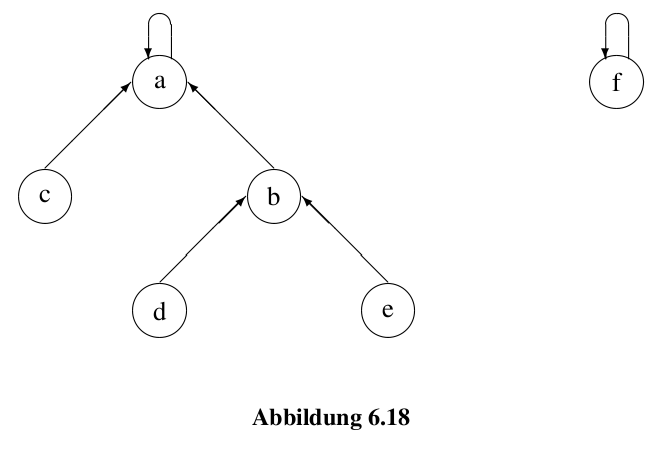
\includegraphics[scale=0.4]{Figures/ufs.png}
\end{center}
Per evitare che un set degeneri ad una lista ci sono due soluzioni: l'unione in base alla grandezza o all'altezza. In entrambi i casi l'idea è di rendere l'albero più piccolo un sottoalbero di quello più grande. Necessitiamo dunque di un altro array in cui viene salvata la grandezza. Per semplicità adottiamo una nomenclatura diretta, vale a dire che un insieme porta il nome del suo primo elemento (radice).
\begin{lstlisting}
int[] size, p //di grandezza n
//elementi da 1 a n

make-set(x)
	p[x]=x
	size[x]=1

union(e,f)
	if size[e]<size[f]
		swap(e,f)
	p[f]=e
	size[e]+=size[f]
	
int find(x)
	int y=x
	while p[y]!=y //non si tratta di una radice
		y=p[y]
	return y			
\end{lstlisting}
\begin{mytheorem}{6.3}
Il processo ``unione per grandezza'' (Vereinigung nach Grösse) conserva la seguente caratteristica: un albero di altezza h ha almeno $2^h$ nodi.
\paragraph*{Dimostrazione}
Ammettiamo che dobbiamo unire gli alberi $T_1 \mbox{ e } T_2$ e che il primo sia più grande del secondo, quindi $g(T_1)\geq g(T_2)$. Secondo l'ipotesi $T_i \mbox{ ha almeno } 2^{h_i}$ nodi. 
\begin{itemize}
\item Caso 1: $altezza(T_1 \cup T_2)=max\{h_1,h_2\}$
Quindi l'altezza dell'unione è per forza almeno $2^{altezza(T_1 \cup T_2)}$.
\item Caso 2: l'altezza del $max\{h_1,h_2\}$ è cresciuta di uno. Questo è possibile solo se $altezza(T_1 \cup T_2)=h_2+1$. Quindi:
$$g(T_1)\geq g(T_2) \geq 2^{h_2} $$
$$g(T_1 \cup T_2)=g(T_1)+g(T_2) \geq 2*2^{h_2}=2^{h_2+1}=2^{altezza(T_1 \cup T_2)}$$
\end{itemize}
\end{mytheorem}
Come diretta conseguenza find(x) impiega al massimo log(n) passi. Le altre operazioni sono fattibili in tempo costante.

\chapter{Geometrische Algorithmen}
\section{Konvexe Hülle (pag 472)}
Di seguito presenterò soltanto la soluzione migliore che si può trovare senza utilizzare il principio Scan line, vale a dire Graham's scan. La Konvexe Hülle altro non è che una figura che contiene tutti i punti (noi siamo interessati nella minima, quindi quella formata da meno segmenti).
\subsection{Graham's scan}
Si sceglie inizialmente un qualsiasi punto (al centro) e si calcolano le equazioni delle rette che connettono il punto scelto con gli altri punti. Dopodiché si ordinano i punti in base all'angolo (dato dalla pendenza), partendo da ore sei e procedendo in senso antiorario (vedi immagine). Dopodiché non rimane che collegare i punti seguendo questo ordine. Dato che siamo interessati alla minima Konvexe Hülle, se un segmento va verso sinistra (in relazione al senso di marcia antiorario) per poi tornare verso destra significa che questi due segmenti possano essere sostituiti da un segmento più lungo. Bisogna in seguito anche ricontrollare i segmenti precedenti. 
\begin{center}
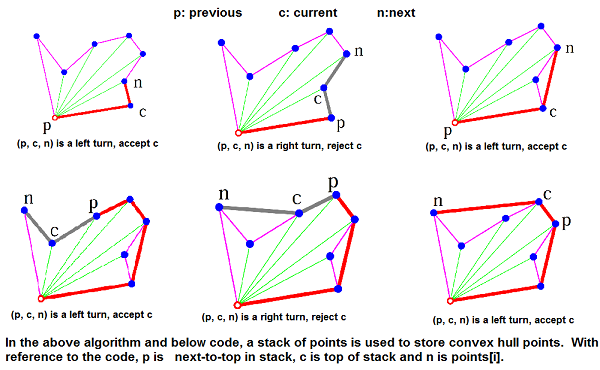
\includegraphics[scale=0.7]{Figures/graham.png}
\end{center}
Secondo l'analisi ammortizzata ogni segmento candidato può essere allontanato al massimo una volta, quindi O(n). Il costo dell'algoritmo è quindi dato dal sort, quindi si tratta di $O(n\log (n))$.

\section{Scan line principle}
\subsection{Il principio (pag 478)}
Il principio consiste nell'analizzare il problema utilizzando una linea verticale (o anche orizzontale), la scan line, che si ferma ad ogni punto discreto analizzando il problema. Risulta quindi necessario ordinare questi punti in base ad una determinata coordinata. La scan line divide gli oggetti geometrici in tre tipi: attivi (sulla scan line), morti(a sinistra) e inattivi (a destra). Di seguito l'algoritmo:
\begin{lstlisting}
	Q=insieme di punti discreti (Haltepunkten)
	L=null //punti attivi
	while !Q.isEmpty()
		//scegli il prossimo punto p da Q ed allontanalo da Q
		update(L,p) //aggiorna gli oggetti attivi
		//risolvi la parte del problema
\end{lstlisting}
\subsection{Sichtbarkeitsproblem (pag 480)}
Come esempio facile osserviamo questo problema. Dato un insieme di segmenti orizzontali ritorna le coppie visibili tra di loro, vale a dire che possono essere collegati da una retta verticale senza che essa si incroci con altri segmenti.
\begin{lstlisting}
Q=punti di inizio e fine segmento ordinati secondo l'asse Ox
L=null
while !Q.isEmpty
	p=Q.next
	if (p punto sinistro del segmento s)
		L.add(s)
		//trova i vicini f e g di s in L
		//ritorna le coppie (s,f) e (s,g)
	else
		//trova i vicini f e g di s in L	
		L.remove(s)
		//ritorna (f,g)
\end{lstlisting}
L'algoritmo impiega $O(n \log (n))$ e uno spazio di O(n).
\subsection{Schnittproblem für iso-orientierte Liniensegmente (pag 483)}
Il problema è quello di trovare i tutti punti di intersezione, dato un disegno composto di segmenti verticali e orizzontali.
\begin{lstlisting}
Q=insieme delle coordinate x dei punti di inizio e di fine dei segmenti
L=null //insieme dei segmenti orizzontali attivi secondo le coordinate y
while !Q.isEmpty
	p=Q.next
	if (p punto sinistro di un segmento orizzontale s)
		L.add(s)
	else if (p punto destro di un segmento orizzontale s)
		L.remove(s)
	else 
		/*p coordinata x di un segmento verticale s con delimitato da
		  (p,yu) e (p,yo) */
		//trova tutti i segmenti t di L con yu<=y(t)<=yo
		//ritorna questi punti   		
\end{lstlisting}
Non ci rimane che trovare la struttura dati ideale per L. Essa deve riuscire ad effettuare delle cosiddette Bereichsanfrage (range query) nel tempo minore possibile. Un'implementazione possibile è quella di organizzare L come un albero AVL in cui le chiavi vengono totalmente salvate nelle foglie (Blattsuchbaum). Inoltre le foglie devono essere collegate da una doppia lista lineare, in modo da poter semplicemente determinare gli elementi tra una chiave ed un'altra.
\todo{Aggiungere immagine a pagina 485}
Una Bereichsanfrage può dunque essere effettuata in $O(\log (n)+r$ passi, dove r è il numero di elementi tra a e b. La soluzione del problema avviene dunque il $O(n\log (n)+k)$ passi, dove k è il numero di segmenti che si incrociano.

\chapter{Graphenalgorithmen}
\section{Topologisches Sortieren (pag 597)}
Topological sort non è altro che la creazione di una relazione di ordine totale a partire da una parziale (esse possono essere rappresentate in forma di grafi e matrici, vedi Diskrete Mathematik). Una relazione di ordine parziale richiede che il grafo non abbia cicli, quindi si presta bene come test a riguardo.
\begin{lstlisting}
ord //array che da un ordine ad ogni nodo

topSortBasic(Graph G)
	int count=0
	while (G ha almeno un nodo v con indeg=0){
		count++
		ord[v]=count
		G=G-v
		}
	if G=null
		//G senza cicli
	else
		//G ha cicli		
\end{lstlisting}
Questa è l'idea di base dell'algoritmo. Per trovare un nuovo nodo col grado di entrata 0 (nella relazione di ordine parziale non ha valori che lo precedono), si può seguire le frecce in ordine opposto partendo da un nodo qualsiasi. In questo modo si impiega $\Omega (n^2)$ passi per l'algoritmo. Una variante più efficiente è la seguente:
\begin{lstlisting}
topSort(Graph G)
	int lfdNr=0
	Stack<Node> degzero
	indeg //array [Node] of integers
	
	//set eingrad[v]
	for v=1:n //assume that G has n nodes
		indeg[v]=0 
		for v=1:n
			p=adjacencyList[v]
			while p!=null
				indeg[p.endnode]++
				p=p.next
	
	//set degzero
	for v=1:n
		if indeg[v]=0
			degzero.push(v)
	
	//topsort
	while degzero!=null
		v=degzero.pop()
		lfdNr++
		ord[v]=lfdNr
		p=adjacencyList[v]
		while p!=null
			w=p.endnode		
			indeg[w]--
			if indeg[w]=0
				degzero.push(w)
	//conditions
	if lfdNr=n
		//cycle free
	else
		//has cycle
									
\end{lstlisting}
L'algoritmo impiega $O(|V|+|E|)$.
\section{Transitive Hülle}
È esattamente la stessa cosa che la transitive closure (matematica discreta, capitolo relazioni). Dato un grafo G come matrice, l'algoritmo ritorna la matrice rappresentante la reflexive and transitive closure. Praticamente se A[i,j]=1 significa che esiste una via da i a j.
\begin{lstlisting}
for i=1:n
	A[i,i]=1
for j=1:n
	for i=1:n
		if A[i,j]==1
			for k=1:n
				if A[j,k]==1
					A[i,k]=1	
\end{lstlisting}
Approssimativamente richiede $O(|V|^3)$, nel dettaglio $O(|V|^2+|E||V|)$.
\section{Search}
\subsection{Breadth first search}
\begin{center}
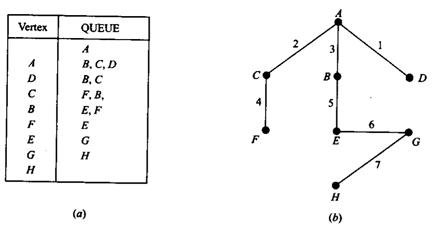
\includegraphics[scale=1]{Figures/bfs.JPG}
\end{center}
Da notare che se al posto della coda si utilizza uno stack si ottiene una depth first search.
\begin{lstlisting}
BFS(Graph G,Vertex v)
     create a queue Q
     create a set V
     enqueue v onto Q
     add v to V
     while Q is not empty loop
     	t=Q.dequeue()
       	if t is what we are looking for 
            	return t
     	for all edges e in G.adjacentEdges(t)
			u = G.adjacentVertex(t,e)
           	if u is not in V
            	   add u to V
            	   enqueue u onto Q           
\end{lstlisting}
L'algoritmo impiega uno spazio di $O(|V|^2)$ e una complessità di $O(|V|+|E|)$. Da notare che ogni nodo viene raggiunto per la miglior via.
\subsection{Depth first search (pag 607)}
Al posto di usare una coda usiamo uno stack. Nel caso di prima l'ordine con cui i lati vengono visitati sarebbe quindi: A, B, E, G, H, C, F, D. Possiamo usare questo algoritmo per apprendere alcune caratteristiche del grafo, quali la suddivisione dei vari tipi di lati. Definiamo l'albero risultate dai lati utilizzati dalla ricerca (Baumpfeile) come DFS-tree. Ad ogni nodo associamo un indice, che rappresenta l'ordine con cui viene visitato. Differenziamo il depth-first-begin-index (DFBI), che rappresenta l'ordine con cui vengono inseriti nello stack, e il depth-first-end-index (DFEI), l'ordine con cui vengono allontanati dallo stack. Definiamo dunque i tipi possibili di lati:
\begin{itemize}
\item Appartenenti al DFS-tree: Baumpfeile.
\item Frecce che arrivano ad un nodo già visitato: Vorwärtspfeile.
\item Frecce che tornano ad un predecessore del DFS-tree: Ruckwärtspfeile.
\item Altrimenti chiamate Seitwärtspfeile.
\end{itemize}
Esempio:
\begin{center}
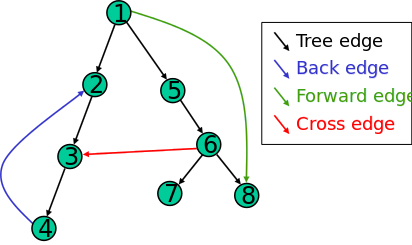
\includegraphics[scale=0.7]{Figures/edgetype.png}
\end{center}
Con l'aiuto di questo algoritmo ricorsivo possiamo arrivare a tutte le informazioni:
\begin{lstlisting}
Set<Vertex> B=nullSet
int dfbi=dfei=0
Set<Edge> BP=VP=RP=SP=nullSet
Graph G
Node start
int[] DFEI,DFBI

public static void main(String[] args)
	DFS(G, start, null)

DFS(Graph G, Node v,w)
	//depth first search, starting from node v, that comes from w
	if !B.has(v)
		//v not reached yet
		B=B+{v} //where + denotes the union of two sets
		BP=BP+{(w,v)}
		dfbi++
		DFBI[v]=dfbi
		for (Edge (v,u):G.E) //G.E=set of edges of G
			DFS(G, u,v)
		dfei++
		DFEI[v]=dfei
	else
		//classify edge
		if DFBI[w]<=DFBI[v]
			//forward edge
			VP=VP+{(w,v)}
		else if DFEI[w]==0 
			//DFS not finished for w, that means w is an ancestor of v
			BP=BP+{(w,v)}
		else
			//cross edge
			SP=SP+{(w,v)}			
\end{lstlisting}
In un grafo non diretto non ci sono cross edges. Interessante notare che invertendo l'ordine del DFEI si ottiene un topological sort (dimostrato in un esercizio, penso accada lo stesso senza invertire il DFBI in un grafo connesso e senza cicli). Un'altra possibile applicazione potrebbe essere quella di ricavare uno spanning tree.\todo{Supposizioni logiche, non sicure e non dimostrate} 
\section{Kürzeste Weg (pag 619)}
Per ogni lato definiamo una funzione c((v,u)) che ne associa il costo.
\subsection{Dijkstra}
Ammettiamo che tutti i costi siano positivi. Se p=(a,...,f) è una via più corta tra a ed f, allora lo devono essere anche tutte le vie intermedie.
\begin{lstlisting}
int infinity //a big number
Set<Node> R=nullSet
	
Dijkstra(Graph G, Node s)
	for (Node v: V-{s})
		v.predecessor=null
		v.distance=infinity
		v.chosen=false	
	s.predecessor=s
	s.distance=0
	s.chosen=true
	//i vertici adiacenti a s appartengono al bordo (Rand)
	fillR(s)
	while !R.isEmpty()
		//scegli v con v.distance minima e allontanalo da R
		v.chosen=true
		fillR(v)
		
fillR(Node v)
	for (Edge (v,u):E)
		if !u.chosen && (v.distance+c((v,u))<u.distance)
			u.predecessor=v
			u.distance=v.distance+c((v,u))
			R.add(u)				
\end{lstlisting}
L'efficienza dell'algoritmo dipende dalla struttura dati rappresentata da R, che necessita di eseguire le seguenti operazioni nel minor tempo possibile:
\begin{enumerate}
\item Inizializzare
\item Controllare se è vuoto
\item Trovare e allontanare il nodo con la distanza minima
\item Aggiungere una nuova voce
\end{enumerate}
Di seguito le possibili implementazioni con i loro costi:
\paragraph*{Non salvarlo esplicitamente}
Inizialmente tutti i nodi che non sono stati scelti appartengono a R. Dopodiché 1. e 4. non devono più essere eseguiti. Per 2. e 3. basta controllare tutti i nodi. Il tempo richiesto dall'algoritmo diventa dunque $O(|V|^2)$, molto efficiente solo se ci sono molti lati.
\paragraph*{Heap}
Le operazioni 1. e 2. richiedono tempo costante, mentre 3. e 4. tempo logaritmico. In totale $O(|E|\log (|V|))$.
\paragraph*{Fibonacci Heap}
1, 2, 4 possono essere eseguite in tempo ammortizzato costante, mentre 3. in tempo logaritmico. In totale $O(|E|+|V|\log (|V|))$.
\subsection*{Bellman-Ford}
Nel caso di un grafo con valori negativi il percorso più breve si lascia trovare nel seguente modo:
\begin{lstlisting}
int infinity //a big number
Set<Node> R=nullSet
	
Dijkstra(Graph G, Node s)
	for (Node v: V-{s})
		v.predecessor=null
		v.distance=infinity
	s.predecessor=s
	s.distance=0
	//i vertici adiacenti a s appartengono al bordo (Rand)
	fillR(s)
	while !R.isEmpty()
		//scegli v allontanalo da R
		fillR(v)
		
fillR(Node v)
	for (Edge (v,u):E)
		if v.distance+c((v,u))<u.distance
			u.predecessor=v
			u.distance=v.distance+c((v,u))
			R.add(u)				
\end{lstlisting}
Attenzione: se c'è un ciclo negativo il processo potrebbe non finire. Altrimenti il tempo impiegato è $O(|V||E|)$.
\begin{lstlisting}
     //controlla la presenza di cicli negativi
     for each arco uv in archi:
        u := uv.source
        v := uv.destination
        if v.distance > u.distance + uv.weight:
           error "Il grafo contiene un ciclo di peso negativo"
\end{lstlisting}
\section{Minimale spannende Baum (pag 631)}
Per risolvere questo problema utilizziamo un procedimento greedy, vale a dire l'applicazione iterativa delle seguenti regole:
\paragraph*{Regola 1} Tra due ``cut'' non connessi scegli l'arco dal costo minore.
\paragraph*{Regola 2} Se ci troviamo in un ciclo, elimina il nodo dal costo maggiore.
\paragraph*{Invariante} L'invariante dell'algoritmo è che l'applicazione di queste regole mantiene il minimum spanning tree parziale minimo. 
\begin{mytheorem}{9.1}
Qualsiasi algoritmo che rispetti le precisazioni fatte sopra garantisce l'invariante.
\paragraph*{Dimostrazione} Fatta in classe e leggibile a pag 629 (abbastanza triviale).
\end{mytheorem}
\subsection{Kruskal}
Il principio dell'algoritmo è semplice: inizialmente ogni nodo rappresenta un albero minimale separato. Dopodiché avviene un'iterazione in base al prezzo degli archi: se l'arco appartiene già a uno dei sottoalberi non viene scelto, altrimenti sì, quindi i due sottoalberi vengono uniti. Per un'efficiente implementazione i lati devono essere ordinati in senso crescente già all'inizio e i nodi vengono salvati in una Union find structure. 
\begin{lstlisting}
Set<Edge> S //solution
UnionFind uf
sort E
for (Vertex v:V)
	uf.makeSet(v)
for (Edge (v,w):E)
	if uf.find(v)!=uf.find(w)
		S.add((v,w))
		uf.union(find(v),find(w))
	
\end{lstlisting}
L'algoritmo impiega $O(|E|\log (|V|))$.
\subsection{Prim,Dijkstra}
Iniziamo con un nodo e finché non siamo alla fine, quindi n-1 passi, scegliamo ogni volta l'arco che possiede un solo nodo nell'albero e con costo minimo. In questo modo impieghiamo $O(|E|+|V|\log (|V|))$.
\section{Flüsse in Netzwerken (pag 637)}
Innanzitutto si cerca una via che collega q a s (Quelle und Senke). Dopodiché si costruisce un cosiddetto Restgraph nel modo seguente:
\begin{center}
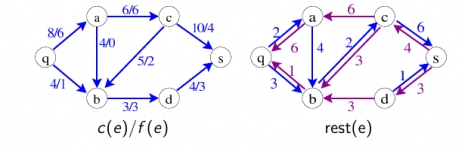
\includegraphics[scale=0.8]{Figures/restgraph.jpg} 
\end{center}
Le frecce viola indicano la capacità utilizzata, mentre quelle blu ciò che ancora rimane. Finché esiste ancora un percorso nel grafo, che può essere trovato ad esempio tramite breadth first search, è ancora possibile aumentare la capacità su quella via. Intuitivamente si può capire che la capacità massima del flusso è limitata dal taglio minimo (min cut), più precisamente essi sono uguali.
\begin{lstlisting}
//initialize
for (Edge e:E)
	f(e)=0
//iterations, the flow f grows up
while (there is a path p from q to s)
	r=min\{rest(e)|e is in p\}
	grow f across p of r units
\end{lstlisting}
Si tratta di una semplice versione che richiede $O(|V||E|^2)$. Tramite l'inserimento di una soglia c approssimativa (Schwelle) che viene dimezzata ad ogni iterazione possiamo migliorarne il tempo. In questo caso consideriamo solo i lati con una capacità maggiore della soglia, aumentiamo la capacità per poi diminuire la soglia. Il tempo richiesto è di $O(\log (c)m^2)$. 

Ecco una versione completa dell'algoritmo di base, estratta dall'API condivisa sul seguente link: \url{https://db.tt/ftsSt6j9}.
\begin{lstlisting}
package GraphAPI;
import java.util.LinkedList;
import DataStructure.Queue;

public class MaxFlow {
	private int infinity=100000000;
    private boolean[] marked;     // marked[v] = true if s->v path in residual Network
    private FlowEdge[] edgeTo;    		// edgeTo[v] = last edge on shortest residual s->v path
    private Network G;
    private int s, t;

    public MaxFlow(Network G, int s, int t) {
    	this.G=G;
    	this.s=s;
    	this.t=t;
    }

    public int compute(){
    	int res=0;
    	while (hasPath()){
    		int min=infinity;
    		//compute the min flow on the residual Network
    		BreadthFirstSearch search=new BreadthFirstSearch(G);
    		Iterable<Integer> path=search.pathToFrom(t,s); //path from s to t
    		for (int e:path)
    			if (edgeTo[e].residualCapacityTo(e)<min)
    				min=edgeTo[e].residualCapacityTo(e);
    		
    		//add min to all edges on the path
    		for (int e: path)
    			edgeTo[e].addResidualFlowTo(e, min);
    		res+=min;
    	}
    	return res;
    }
  
    private boolean hasPath(){
    	edgeTo=new FlowEdge[G.V()];
    	marked=new boolean[G.V()];
    	
    	Queue<Integer> q=new Queue<Integer>();
    	q.enqueue(s);
    	while(!q.isEmpty()){
    		int v=q.dequeue();
    		marked[v]=true;
    		for (FlowEdge e : G.adj(v)){
    			int w=e.other(v);
    			if (e.residualCapacityTo(w)>0 && !marked[w]){
    				edgeTo[w]=e;
    				q.enqueue(w);
    			}
    		}
    	}
    	return marked[t];
    }
    
    public Iterable<Integer> path(){
    	LinkedList<Integer> path=new LinkedList<Integer>();
    	int pos=t;
    	while (pos!=s){
    		path.addFirst(pos);
    		pos=edgeTo[pos].other(pos);
     	}
    	return path;
    }
}
\end{lstlisting} 
\subsection{Maximale Zuordnung in bipartiten Graphen (pag 646)}
Consideriamo il problema del matching ottimale tra due set. Le coppie possibili possono essere semplicemente modellate come un grafo bipartito, che a sua volta può essere trasformato nella forma utilizzata per i flussi:
\begin{center}
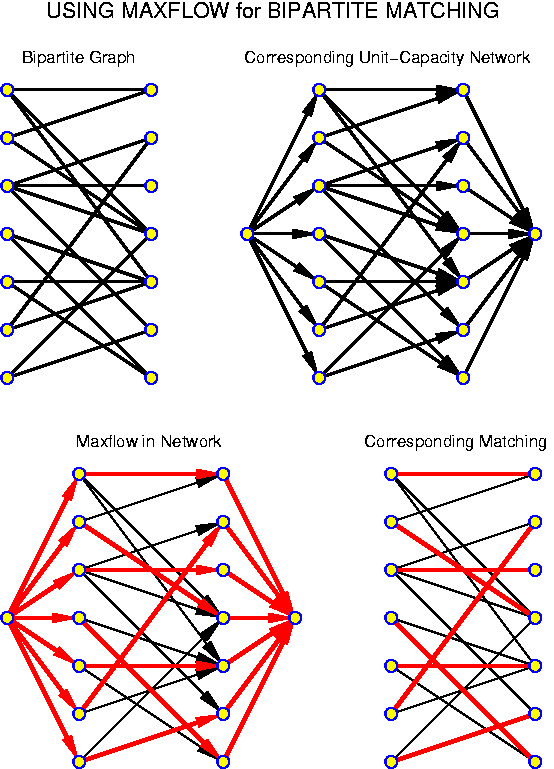
\includegraphics[scale=0.5]{Figures/matching.jpg}
\end{center}
In questo caso, dato che il costo è sempre 1, la crescita del Restgraph consiste semplicemente nel cambiamento di direzione delle frecce. In un livello di astrazione più concreto questo corrisponde nel liberare una coppia per poterne formare altre due. L'esecuzione dell'algoritmo in questo speciale tipo di grafo richiede solamente $O(\sqrt{|V|}|E|)$.
\end{document}
